\documentclass[conference]{IEEEtran}
\IEEEoverridecommandlockouts
% The preceding line is only needed to identify funding in the first footnote. If that is unneeded, please comment it out.
\usepackage{acronym}

\usepackage{esvect}

\acrodef{PSO}[PSO]{\emph{particle swarm optimisation algorithm}}
\acrodef{NN}[NN]{\emph{neural network}}
\acrodef{CPSO}[CPSO]{\emph{chaotic particle swarm optimisation algorithm}}
\acrodef{RNG}[RNG]{\emph{random number generator}}
\acrodef{CPRNG}[CPRNG]{\emph{chaotic pseudo-random number generator}}
\acrodef{VN}[VN]{\emph{Von Neumann}}
\acrodef{MSE}[MSE]{\emph{mean squared error}}
\usepackage{cite}
\usepackage{amsmath,amssymb,amsfonts}
\usepackage{commath}
\usepackage{algorithmic}
\usepackage{array,multirow,graphicx}
\usepackage{textcomp}
\def\BibTeX{{\rm B\kern-.05em{\sc i\kern-.025em b}\kern-.08em
    T\kern-.1667em\lower.7ex\hbox{E}\kern-.125emX}}
\begin{document}

\title{Investigating Chaotic Particle Swarm Optimisation for Neural Network Training\\
}

\author{\IEEEauthorblockN{\\Quinton Weenink}
\IEEEauthorblockA{\textit{dept. Computer Science} \\
\textit{University of Pretoria}\\
Pretoria, South Africa \\
u13176545@tuks.co.za}
\and
Supervisor:\\
\IEEEauthorblockN{Ms. Anna Bosman}
\IEEEauthorblockA{\textit{dept. Computer Science} \\
\textit{University of Pretoria}\\
Pretoria, South Africa \\
annar@cs.up.ac.za}
}

\maketitle

\begin{abstract}
Historically, particle swarm optimisation algorithms have been successfully applied to neural network training, sometimes outperforming traditional gradient-based approaches. Studies have however shown that particle swarm optimisation algorithms do not scale very well, performing poorly on high-dimensional neural network architectures. This study aims to investigate the effect of using the chaotic particle swarm optimisation algorithm for neural network training. Observing that chaotic maps do not always beneficially influence neural network training in a constantly significant manner.
\end{abstract}

\begin{IEEEkeywords}
CPSO, NN, Chaotic
\end{IEEEkeywords}

\section{Introduction}
Chaotic maps are mathematical maps or evolution functions that exhibit some sort of chaotic behaviour. A \ac{CPSO} is a \ac{PSO} that makes use of a chaotic map as part of its implementation. There are different methods that all borrow from the same idea of applying the chaotic maps to the standard \ac{PSO} algorithm  \cite{pluhacek:cpso-iw, pluhacek:cpso-cprng-imp}. One of the best performing \ac{CPSO} implementations uses a \ac{CPRNG} for the random numbers required by the \ac{PSO}. The velocity for a particle is influenced by the chosen \ac{RNG}. Due to this, it can be hypothesised that the chosen \ac{RNG} could have a significant influence on the \ac{PSO}'s performance \cite{pluhacek:cpso-cprng-imp}.

While studies have been conducted on \ac{PSO} trained \ac{NN}s \cite{vanwyk:overfitting-psoffnn, anna:saturation-psonn, anna:meas-sat-nn}, as well as the performance of \ac{CPSO}s \cite{pluhacek:cpso-cprng-imp, pluhacek:cpso-esb-chaotic}, none have been found to investigate the influence of \ac{CPSO} trained \ac{NN}s. Performance as well as overfitting remains a gap in the field of \ac{CPSO}s. While results do look positive for most applications of \ac{CPSO}s these implementations were applied to specific situations that may not be a clear indication of \ac{CPSO} being beneficial to all \ac{NN} training.

This research aims to determine hwo the performance of a \ac{CPSO} compaires to that of the \ac{PSO}, described by Kennedy and Eberhart in \cite{kennedy:pso}, for \ac{NN} training. In completing this research the understanding of \ac{CPSO}s as well as their effectiveness they have on \ac{NN} training will be improved. Additionally, this research aims to assist others when training \ac{NN}s with \ac{CPSO}s.

\section{Particle Swarm Optimization}
A \ac{PSO} is a machine learning algorithm where each particle in the population represents a possible solution to the optimisation problem \cite{anna:meas-sat-nn}. Each particle moves around the search space attempting to find the optimal solution with the influence of its neighbouring particles. The position for each particle iteration is calculated as follows.

\begin{equation} \label{eq:pso:update-position}
\vec{x}_{i}^{\,t} = \vec{x}_{i}^{\,t-1} + \vec{v}_{i}^{\,t}
\end{equation}

\noindent Where:
\begin{itemize}
	\item $ \vec{x} $ is the particle position vector in n-dimensions
	\item $ \vec{v} $ is the particle velocity vector, used to calculate the particles next position
	\item $t$ is the time increment
	\item $i$ is the particle number
\end{itemize}
\vspace{5mm}
\noindent For each iteration of the algorithm, a new location of the particle is calculated based on its previous location and velocity vector as seen in (\ref{eq:pso:update-position}). The following describes a the velocity update algorithm.

\begin{equation} \label{eq:pso:update-velocity}
\vec{v}_{i}^{\,t} = w . \vec{v}_{i}^{\,t-1} + c_1 . \vec{r}_{1}^{\,t} . (\vec{x}_{pBest, i} - \vec{x}_{i}^{t-1}) + c_2 . \vec{r}_{2}^{\,t} . (\vec{x}_{nBest, i} - \vec{x}_{i}^{t-1})
\end{equation}

\noindent Where:
\begin{itemize}
	\item $c_1$ is the acceleration coefficient for the cognitive component
	\item $c_2$ is the acceleration coefficient for the social component
	\item $r_1$ and $r_2$ is a vector of random numbers in the range (0, 1)
	\item $\vec{x}_{pBest}$ is the personal best position of that particle
	\item $\vec{x}_{nBest}$ is the best position found in that particles neighbourhood
\end{itemize}
\vspace{5mm}
\noindent Particle's social component, the third term in (\ref{eq:pso:update-velocity}), requires $ nBest $, the best neighbouring particles position. The set of neighbouring particles is determined by the topology used in the \ac{PSO}. Different topologies could influence the performance of the \ac{PSO}.

Additionally, velocity max, $ V_{max} $, can be used as the limiter when calculating the particle's velocity in (\ref{eq:pso:update-velocity}), ensuring that the particle stays inside search space as well as reduce skipping over more optimal solutions. $ V_{max} $ could however prevent particles from exploring more optimal solutions.

    \subsection{Social Network Topologies}
    
    In the above mentioned \ac{PSO} the neighbourhood could be described in a variety of ways. One such method is the $ gBest $ topology, where each particle is a neighbour of every other particle in the network. This means that the particle's $ nBest $ is always the global best particle for the swarm. 
    
    Another social topology called $ lBest $ connects particles in a ring topology, the neighbourhood is specified by a fixed size of $ n_s $. The $ nBest $ in this case is determined by the best particle within $ n_s $ neighbours from the current particle\cite{vanwyk:overfitting-psoffnn}. 
    
    Finally, another social network topology exists called the \ac{VN} social network topology. This topology connects each particle to its neighbours in a lattice\cite{vanwyk:overfitting-psoffnn}. In order to determine the $ nBest $, the best error of its north, south, east and western, neighbours is used (\ref{eq:pso:update-velocity}).
    
    
\section{Chaotic Maps and \ac{CPRNG}s}
	For this research, it was decided to implement the \ac{CPSO} using a \ac{CPRNG} due to previous studies indicating the better performance of such an implementation \cite{pluhacek:cpso-cprng-imp}\cite{pluhacek:cpso-esb-chaotic}. Other implementations include using chaotic maps to place particles in the search space.
	
	All the chaotic map's initial $ X_0 $ and $ Y_0 $ were sampled in a uniform distribution $ (0, 1) $ unless stated otherwise.
	
	Each of the following maps were iteratively sampled from the chaotic maps listed bellow over 5000 iterations. Each batch was then scaled from (0, 1) as required by the \ac{PSO} for $ r_1 $ and $ r_2 $ in Equation (\ref{eq:pso:update-velocity}).
	
	\subsection{Tinkerbell map}
	
	The Tinkerbell map (depicted in Fig. \ref{fig:map:tinkerbell}) is a two-dimensional complex discrete-time dynamical system given by Eqs. (\ref{eq:tinkerbell:x}) and (\ref{eq:tinkerbell:y}).
	
	Due to the potentially exponential nature of the algorithm the initial $ X_n $ and $ Y_0 $ had to be randomly distributed to $ -(0.01, 0.1) $ and $ (0, 0.1) $ respectively.
	
	\begin{equation} \label{eq:tinkerbell:x}
	X_{x+1} = X_n^2 - Y_n^2 + aX_n + bY_n
	\end{equation}
	\begin{equation} \label{eq:tinkerbell:y}
	Y_{n+1} = 2X_nY_n cX_n + dY_n
	\end{equation}

    \noindent The following parameters were used in this research: $ a = 0.9 $ and $ b = -0.6 $ used in (\ref{eq:tinkerbell:x}) as well as $ c = 2 $ and $ d = 0.5 $ used in (\ref{eq:tinkerbell:y}) as suggested in \cite{pluhacek:cpso-cprng-imp}.
    \vspace{5mm}
    
    \begin{figure}[htbp]
\centerline{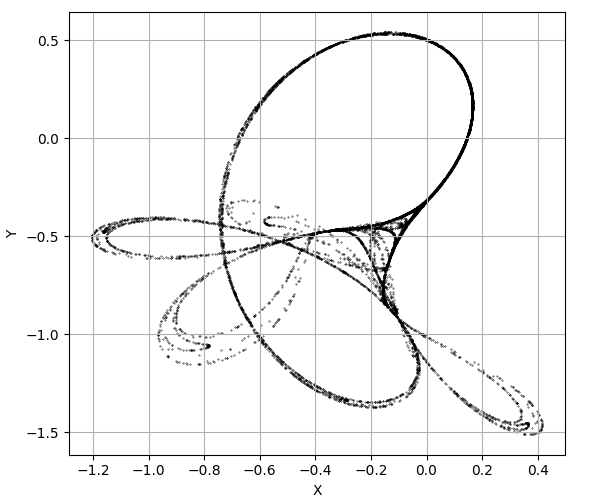
\includegraphics[width=90mm]{images/maps/Tinkerbell.png}}
\caption{Tinkerbell map}
\label{fig:map:tinkerbell}
\end{figure}
	
	\subsection{Lozi map}
	Depicted in Fig. \ref{fig:map:lozi}, the Lozi map is a simple discrete two-dimensional chaotic map. The map equations are given in \ref{eq:lozi:x} and \ref{eq:lozi:y}.
	
	\begin{equation} \label{eq:lozi:x}
	X_{x+1} = 1 - a \abs{X_n} + bY_n
	\end{equation}
	\begin{equation} \label{eq:lozi:y}
	Y_{n+1} = X_n
	\end{equation}

	\noindent The parameters used in (\ref{eq:lozi:x}) for this work are: $ a = 1.7 $ and $ b = 0.5 $ as suggested in \cite{pluhacek:cpso-cprng-imp}.
	\vspace{5mm}
	
	\begin{figure}[htbp]
\centerline{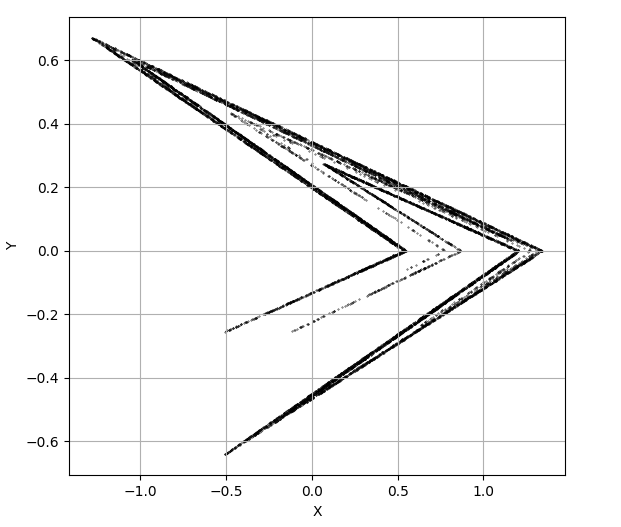
\includegraphics[width=90mm]{images/maps/Lozi.png}}
\caption{Lozi map}
\label{fig:map:lozi}
\end{figure}
	
	\subsection{Dissipative standard map}
	
	The Dissipative standard map is a two-dimensional chaotic map \cite{pluhacek:cpso-cprng-imp}. The Dissipative standard map is given in Fig. \ref{fig:map:dissipative} with the map equations are given in Eqs. (\ref{eq:dissipative:x}) and (\ref{eq:dissipative:y}).

    Observing the results of \cite{pluhacek:cpso-iw} one can hypothesise that the Dissipative standard map would perform better in higher dimentional problems.
	
	\begin{equation} \label{eq:dissipative:x}
	X_{x+1} = X_n + Y_{n+1} (mod 2\pi)
	\end{equation}
	\begin{equation} \label{eq:dissipative:y}
	Y_{n+1} = bY_n + k sin X_n (mod 2\pi)
	\end{equation}

	\noindent The constants used in this work are $ b = 0.6 $ and $ k = 8.8 $ in (\ref{eq:dissipative:y}) based on previous experiments \cite{pluhacek:cpso-cprng-imp}.
	
	\begin{figure}[htbp]
\centerline{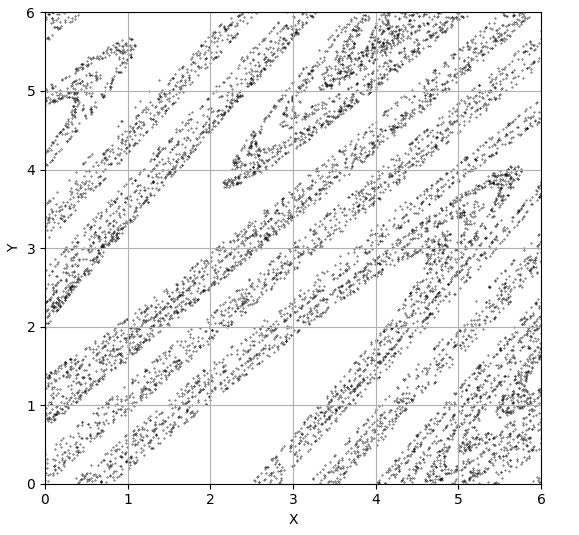
\includegraphics[width=90mm]{images/maps/Dissipative.png}}
\caption{Dissipative standard map}
\label{fig:map:dissipative}
\end{figure}

    
\section{\ac{CPSO}}
Historically, \ac{PSO}s have been successfully applied to \ac{NN} training, sometimes outperforming traditional gradient-based approaches \cite{anna:saturation-psonn, anna:meas-sat-nn}. Studies have however shown that \ac{PSO}s do not scale very well, performing poorly on high-dimensional \ac{NN} architectures. This is as a result of high-dimensionality of the \ac{PSO}'s search space, an inherent property of \ac{NN}s where the number of weights increases exponentially with the linear increase of architecture \cite{anna:saturation-psonn}. 

A \ac{CPSO} is a \ac{PSO} that makes use of the \ac{CPRNG} to generate $ \vec{r}_{1} $ and $ \vec{r}_{2} $ when calculating the particle's velocity in (\ref{eq:pso:update-velocity}). The \ac{CPRNG} will use a chaotic map in order to calculate the generate the random number vectors.

While the work by Pluhacek et al. has proven that \ac{CPSO}s offer better performance over standard \ac{PSO}s in a number of cases \cite{pluhacek:cpso-cprng-imp, pluhacek:ms-cpso, pluhacek:cpso-esb-chaotic}, it is not safe to conclude that \ac{PSO} \ac{NN} training will be improved in general.  Additionally, research has not explored precisely when to use which chaotic map. Some research \cite{pluhacek:cpso-esb-chaotic, pluhacek:ms-cpso} attempts to solve this problem by using a multi-\ac{CPSO} or an ensemble of \ac{CPSO}s with the aim to design universally usable \ac{CPSO}s that will not suffer from some disadvantages of previous \ac{CPSO} designs \cite{pluhacek:pso-mutichaotic-ng}.

\subsection{Neural Network}
Typically, feedforward \ac{NN}s are comprised of neurons connected in layers. Signals travel from the input layer through the hidden layer(s) to the output layer \cite{anna:meas-sat-nn}. Each neuron is connected through a collection of weights to the neurons in the next layer as can be seen in Fig. \ref{fig:nn:configuration}. This study used a \ac{NN} with bias on every layer except the output layer.

    	\begin{figure}[htbp]
\centerline{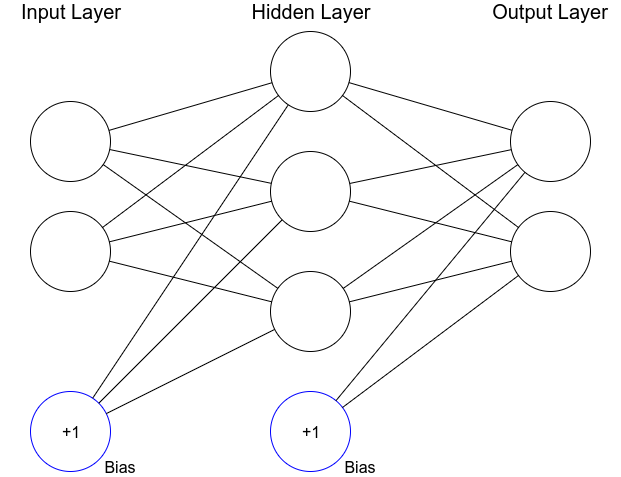
\includegraphics[width=70mm]{images/nn/NeuralNetwork.png}}
\caption{Neural network with bias}
\label{fig:nn:configuration}
\end{figure}

    Back propagation is an often used training method for \ac{NN}s and makes use of forward propagation to generate the \ac{NN}'s output value(s). The weights are manipulated to train the network using the training error.
	
	\begin{equation} \label{eq:nn:sigmoid}
g(net) = \frac{1}{1 - e^{-net}}
\end{equation}
	
	\begin{figure}[htbp]
\centerline{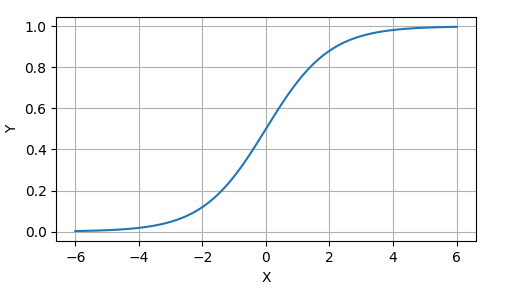
\includegraphics[width=70mm]{images/nn/Sigmoid.png}}
\caption{Sigmoid activation function}
\label{fig:nn:sigmoid}
\end{figure}

    Fig. (\ref{fig:nn:sigmoid}) represents the output of a sigmoid function (\ref{eq:nn:sigmoid}) which will be used as the activation function for \ac{NN}s in this this research.     

	\subsection{PSO trained NN}
	The goal of training a \ac{NN} with a \ac{PSO} is to find an optimal set of weights for the \ac{NN}. The \ac{NN}’s weights are represented by the \ac{PSO}'s dimensions. Each particle represents a \ac{NN} which could be a possible solution. The particle's fitness is determined by the accuracy of its resulting \ac{NN}.
    
    \begin{table}[htbp]
    \caption{PSO dimentions for each data set}
    \begin{center}
    \begin{tabular}{|c|c|}
    \hline
    \textbf{Data Set}& \textbf{\textit{Dimensions}}\\
    \hline
    Glass Identification& 198\\
    \hline
    Iris& 67\\
    \hline
    Wine& 173\\
    \hline
    Prima Indians Diabetes& 222\\
    \hline
    Cleveland Heart& 195\\
    \hline
    \end{tabular}
    \label{tab:pso:dimensions}
    \end{center}
    \end{table}
    
    This research hopes to determine weather the influence of a \ac{CPRNG} allows the trained \ac{NN} to perform better even when \ac{NN} dimensions increase. The number of dimensions each of the particles will navigate is depicted in Table \ref{tab:pso:dimensions}.

	\subsection{Data sets selection and preparation}
	The selection of data sets were based on previous studies that were done on \ac{PSO} training \ac{NN} performance \cite{anna:saturation-psonn, vanwyk:overfitting-psoffnn}. Well known and documented previous studies that show the resulting performance on that data set will also been chosen as a secondary control to measure performance against.
	
	All input to the \ac{NN} was scaled to the range $ [-1, 1] $. While all classification output was mapped to either $ 0.1 $ or $ 0.9 $.
	
	$ D_T $ was measured as $ \frac{2}{3} $ of the total data set and the remainder was allocated to $ D_G $.
	
	\begin{table}[htbp]
    \caption{Neual network configuration for data sets}
    \begin{center}
    \begin{tabular}{|c|c|c|c|c|}
    \hline
    \textbf{Data Set}& \textbf{\textit{Input}}& \textbf{\textit{Hidden}}& \textbf{\textit{Output}}& \textbf{\textit{Source}}\\
    \hline
    Glass Identification& 9& 12& 6& UCI MLR\cite{uci:mlr}\\
    \hline
    Iris& 4& 8& 3& UCI MLR\cite{uci:mlr}\\
    \hline
    Wine& 13& 10& 3& UCI MLR\cite{uci:mlr}\\
    \hline
    Pima Indians Diabetes& 8& 20& 2& UCI MLR\cite{uci:mlr}\\
    \hline
    Cleveland Heart& 13& 10& 5& UCI MLR\cite{uci:mlr}\\
    \hline
    \end{tabular}
    \label{tab:nn:configuration}
    \end{center}
    \end{table}

\section{Measuring performance}

\ac{NN} accuracy is used to determine whether \ac{CPSO} training has improved results over standard \ac{PSO} training. The training error, $ E_T $, was used in order to assess the resulting \ac{NN} accuracy. The training error is calculated as the \ac{MSE} over the training set $ D_T $ of size $ P_T $ represented in (\ref{eq:mse}) \cite{vanwyk:overfitting-psoffnn}.

\begin{equation} \label{eq:mse}
E_{T} = \frac{\sum_{p=1}^{P_{T}}\sum_{k=1}^{K}(t_{k,p}-o_{k,p})^{2}}{P_{T}K}
\end{equation}

Similarly to the training error the generalisation error, $ E_G $, can be used to calculate the performance of the \ac{NN} on the set $ D_G $.

Additionally the generalisation factor $ \rho_F = \frac{E_G}{E_T} $ was also used to measure the overfitting of the trained \ac{NN}s. Each \ac{NN} was trained over 5000 iterations of the \ac{PSO}'s algorithm. A $ \rho_F > 1 $ would indicate a possibility of overfitting due to the generalisation error being greater than the training error. While a $ \rho_f < 1 $ or $ E_G < E_T $ could indicate a lack of overfitting.

\section{Experiments}
    \subsection{\ac{CPRNG} configuration}
    In order to achieve viable results, each experiment was run as a mean over 30 samples. A control was run with a \ac{PSO} that uses a standard \ac{RNG} with $r_1$ and $r_2$ sampled from a uniform distribution $ (0, 1) $ as specified in equation \ref{eq:pso:update-velocity}. The overfitting and performance of the control was measured as a reference. The \ac{CPSO}s will also be observed in the same manner.
    
    For each result observed the only change was a different \ac{RNG} and therefor any significant repeatable performance change measured could be assumed to be the result of this change.
    
    \subsection{\ac{PSO} configuration}
    Both the \ac{VN} and $ gBest $ social network topologies were used for this study. The $ gBest $ \ac{PSO} used $ 25 $ particles, while the \ac{VN} \ac{PSO} used a $ 5 $ by $ 5 $ lattice of $ 25 $ particles.

\section{Results}

The resulting $ E_T $, $ E_G $ and $ \rho_F $ for all experiments conducted in this study are given in Tables \ref{tab:glass}, \ref{tab:iris}, \ref{tab:wine}, \ref{tab:diabetes} and \ref{tab:heart}.

Observing $ \rho_F $ over the results one can see the \ac{CPSO}s, while often outperforming \ac{PSO}, result in a \ac{NN} with higher overfitting. A good depiction of this is the \ac{CPSO}'s performance on the Iris problem. The randomly sampled \ac{PSO} does not perform as well in training, but, results in a \ac{NN} that appears to have less overfitting.

\ac{CPSO}s can be observed to perform well for problems that have a higher error at the end of training, this is were some of the \ac{CPSO}'s performance become more evident. As can be observed in result Tables, the smaller the error the less likely the \ac{CPSO}s will result in a distinguishable performance increase over the randomly sampled \ac{PSO}.

Over all results the Lozi and Tinkerbell chaotic maps \ac{CPSO} perform best on the problems resulting in a \ac{NN}s with less overfitting and higher $ E_G $ than the Dissipative standard map. The dissipative standard map did not perform well in most circumstances contrary what was hypothesised, performing poorly in overall.


\begin{table}[htbp]
\caption{Glass Results after 5000 iterations. Means are reported over 30 samples with standard deviations in parenthesis}
\begin{center}
\begin{tabular}{|c|c|l|l|l|l|}
\hline
\multicolumn{6}{|c|}{\multirow{2}{*}{$ gBest $ topology}}{}\\
\multicolumn{6}{|c|}{}\\
\hline
\multicolumn{2}{|c|}{} & \textbf{\textit{Tinkerbell}} & \textbf{\textit{Lozi}} & \textbf{\textit{Dissipative}} & \textbf{\textit{Uniform}}\\
\hline
\parbox[t]{2mm}{\multirow{6}{*}{\rotatebox[origin=c]{90}{No $ V_{max} $}}}
& \multirow{2}{*}{$ E_T $}
& 0.04525184 & 0.04510496 & \textbf{0.04380078} & 0.04924612\\
& & (0.008998) & (0.015825) & (0.011896) & (0.014376)\\
\cline{2-6}
& \multirow{2}{*}{$ E_G $} 
& \textbf{0.07788302} & 0.07928021 & 0.07839134 & 0.08072251\\
& & (0.006962) & (0.011482) & (0.012285) & (0.017275)\\
\cline{2-6}
& \multirow{2}{*}{$ \rho_F $} 
& 1.76569666 & 1.88129248 & 1.87329206 & \textbf{1.69060593}\\
& & (0.267126) & (0.444181) & (0.433689) & (0.307194)\\
\hline
\parbox[t]{2mm}{\multirow{6}{*}{\rotatebox[origin=c]{90}{$ V_{max} = 0.1$}}}
& \multirow{2}{*}{$ E_T $}
& 0.02331139 & \textbf{0.02245534} & 0.02349460 & 0.02298055\\
& & (0.003019) & (0.002702) & (0.002779) & (0.002288)\\
\cline{2-6}
& \multirow{2}{*}{$ E_G $} 
& 0.05786972 & 0.05928630 & \textbf{0.05754601} & 0.05945405\\
& & (0.002911) & (0.007112) & (0.005912) & (0.005653)\\
\cline{2-6}
& \multirow{2}{*}{$ \rho_F $} 
& 2.52469112 & 2.68452969 & \textbf{2.49401208} & 2.62478755\\
& & (0.350592) & (0.486994) & (0.443459) & (0.455448)\\
\hline
\multicolumn{6}{|c|}{\multirow{2}{*}{Von Neumann topology}}{}\\
\multicolumn{6}{|c|}{}\\
\hline
\multicolumn{2}{|c|}{} & \textbf{\textit{Tinkerbell}} & \textbf{\textit{Lozi}} & \textbf{\textit{Dissipative}} & \textbf{\textit{Uniform}}\\
\hline
\parbox[t]{2mm}{\multirow{6}{*}{\rotatebox[origin=c]{90}{No $ V_{max}$}}}
& \multirow{2}{*}{$ E_T $}
& 0.06762034 & 0.06843397 & 0.07169069 & \textbf{0.06717697}\\
& & (0.009678) & (0.006862) & (0.012895) & (0.008959)\\
\cline{2-6}
& \multirow{2}{*}{$ E_G $} 
& 0.08771098 & 0.08637538 & 0.09128531 & \textbf{0.08421155}\\
& & (0.013657) & (0.009285) & (0.014901) & (0.013971)\\
\cline{2-6}
& \multirow{2}{*}{$ \rho_F $} 
& 1.31367391 & 1.27970440 & 1.29537791 & \textbf{1.26422974}\\
& & (0.215528) & (0.222547) & (0.223924) & (0.207465)\\
\hline
\parbox[t]{2mm}{\multirow{6}{*}{\rotatebox[origin=c]{90}{$ V_{max} = 0.1$}}}
& \multirow{2}{*}{$ E_T $}
& 0.06103854 & \textbf{0.06080808} & 0.06242042 & 0.06300097\\
& & (0.004123) & (0.005100) & (0.004804) & (0.006018)\\
\cline{2-6}
& \multirow{2}{*}{$ E_G $} 
& 0.08317552 & \textbf{0.08229008} & 0.08453649 & 0.08566786\\
& & (0.007380) & (0.008072) & (0.007668) & (0.010444)\\
\cline{2-6}
& \multirow{2}{*}{$ \rho_F $} 
& 1.37143484 & \textbf{1.36674597} & 1.36708748 & 1.37221453\\
& & (0.169578) & (0.203229) & (0.196021) & (0.214361)\\
\hline
\end{tabular}
\label{tab:glass}
\end{center}
\end{table}

The results in Table \ref{tab:glass}, specifically the results where $ V_{max} = 0.1$ is applied with a \ac{VN} topology, represent a relatively consistent performance increase across most problems for \ac{CPSO}s over uniform \ac{PSO}s. The Lozi map \ac{CPSO} outperforms the basic \ac{PSO} as well as the Tinkerbell and Dissipative map \ac{CPSO}.

\begin{table}[htbp]
\caption{Iris Results after 5000 iterations. Means are reported over 30 samples with standard deviations in parenthesis}
\begin{center}
\begin{tabular}{|c|c|l|l|l|l|}
\hline
\multicolumn{6}{|c|}{\multirow{2}{*}{$ gBest $ topology}}{}\\
\multicolumn{6}{|c|}{}\\
\hline
\multicolumn{2}{|c|}{} & \textbf{\textit{Tinkerbell}} & \textbf{\textit{Lozi}} & \textbf{\textit{Dissipative}} & \textbf{\textit{Uniform}}\\
\hline
\parbox[t]{2mm}{\multirow{6}{*}{\rotatebox[origin=c]{90}{No $ V_{max} $}}}
& \multirow{2}{*}{$ E_T $}
& \textbf{0.00431351} & 0.00482629 & 0.00535656 & 0.01033975\\
& & (0.001897) & (0.002183) & (0.002888) & (0.021587)\\
\cline{2-6}
& \multirow{2}{*}{$ E_G $} 
& 0.02731797 & \textbf{0.02433567} & 0.02660090 & 0.02743795\\
& & (0.013110) & (0.008977) & (0.013168) & (0.027432)\\
\cline{2-6}
& \multirow{2}{*}{$ \rho_F $}
& 7.26520511 & 7.16758581 & 6.56600247 & \textbf{6.56074316}\\
& & (3.846323) & (5.888420) & (5.101546) & (5.836499)\\
\hline
\parbox[t]{2mm}{\multirow{6}{*}{\rotatebox[origin=c]{90}{$ V_{max} = 0.1$}}}
& \multirow{2}{*}{$ E_T $}
& 0.00214609 & \textbf{0.00174290} & 0.00177659 & 0.00253293\\
& & (0.001303) & (0.001365) & (0.001019) & (0.001785)\\
\cline{2-6}
& \multirow{2}{*}{$ E_G $} 
& 0.02028782 & 0.01923971 & 0.01989378 & \textbf{0.01713263}\\
& & (0.008862) & (0.007656) & (0.008261) & (0.006033)\\
\cline{2-6}
& \multirow{2}{*}{$ \rho_F $} 
& 14.9864899 & 20.0014144 & 16.5758342 & \textbf{13.4835849}\\
& & (11.49917) & (16.22635) & (13.25325) & (13.07027)\\
\hline
\multicolumn{6}{|c|}{\multirow{2}{*}{Von Neumann topology}}{}\\
\multicolumn{6}{|c|}{}\\
\hline
\multicolumn{2}{|c|}{} & \textbf{\textit{Tinkerbell}} & \textbf{\textit{Lozi}} & \textbf{\textit{Dissipative}} & \textbf{\textit{Uniform}}\\
\hline
\parbox[t]{2mm}{\multirow{6}{*}{\rotatebox[origin=c]{90}{No $ V_{max}$}}}
& \multirow{2}{*}{$ E_T $}
& 0.02306107 & 0.02041756 & 0.02065217 & \textbf{0.01862638}\\
& & (0.009922) & (0.008811) & (0.005960) & (0.006903)\\
\cline{2-6}
& \multirow{2}{*}{$ E_G $} 
& 0.02506312 & 0.02369337 & 0.02377297 & \textbf{0.01938869}\\
& & (0.013233) & (0.009089) & (0.006519) & (0.007605)\\
\cline{2-6}
& \multirow{2}{*}{$ \rho_F $} 
& 1.11893239 & 1.25016177 & 1.21050577 & \textbf{1.11046472}\\
& & (0.493708) & (0.443750) & (0.361705) & (0.414793)\\
\hline
\parbox[t]{2mm}{\multirow{6}{*}{\rotatebox[origin=c]{90}{$ V_{max} = 0.1$}}}
& \multirow{2}{*}{$ E_T $}
& 0.00921532 & 0.00833094 & \textbf{0.00829776} & 0.00886477\\
& & (0.003167) & (0.003190) & (0.003227) & (0.003080)\\
\cline{2-6}
& \multirow{2}{*}{$ E_G $} 
& \textbf{0.01661334} & 0.01842011 & 0.01765593 & 0.01706100\\
& & (0.007306) & (0.007896) & (0.008138) & (0.007613)\\
\cline{2-6}
& \multirow{2}{*}{$ \rho_F $} 
& \textbf{2.61792201} & 3.09107570 & 3.07521083 & 2.68828159\\
& & (2.726593) & (2.736109) & (2.775890) & (2.436320)\\
\hline
\end{tabular}
\label{tab:iris}
\end{center}
\end{table}

Both Tables \ref{tab:glass} and \ref{tab:iris} are a good case for observing the converse of above. The basic \ac{PSO} almost always outperforms all \ac{CPSO}s across almost all data sets. This again pertains to the experiment using the \ac{VN} topology but differs with the use of no $ V_{max} $ restriction.

\begin{table}[htbp]
\caption{Wine Results after 5000 iterations. Means are reported over 30 samples with standard deviations in parenthesis}
\begin{center}
\begin{tabular}{|c|c|l|l|l|l|}
\hline
\multicolumn{6}{|c|}{\multirow{2}{*}{$ gBest $ topology}}{}\\
\multicolumn{6}{|c|}{}\\
\hline
\multicolumn{2}{|c|}{} & \textbf{\textit{Tinkerbell}} & \textbf{\textit{Lozi}} & \textbf{\textit{Dissipative}} & \textbf{\textit{Uniform}}\\
\hline
\parbox[t]{2mm}{\multirow{6}{*}{\rotatebox[origin=c]{90}{No $ V_{max} $}}}
& \multirow{2}{*}{$ E_T $}
& \textbf{0.00447088} & 0.00506288 & 0.00562712 & 0.00449492\\
& & (0.002862) & (0.001890) & (0.003118) & (0.003527)\\
\cline{2-6}
& \multirow{2}{*}{$ E_G $} 
& 0.04408335 & 0.04304486 & 0.04197183 & \textbf{0.04257008}\\
& & (0.018709) & (0.015388) & (0.018403) & (0.014548)\\
\cline{2-6}
& \multirow{2}{*}{$ \rho_F $} 
& 27.0083903 & \textbf{10.2892335} & 15.1338175 & 66.8660072\\
& & (55.44730) & (6.925383) & (27.61655) & (192.1733)\\
\hline
\parbox[t]{2mm}{\multirow{6}{*}{\rotatebox[origin=c]{90}{$ V_{max} = 0.1$}}}
& \multirow{2}{*}{$ E_T $}
& 2.62E-05 & 2.05E-05 & \textbf{1.81E-05} & 2.33E-05\\
& & (2.19E-05 & (1.54E-05 & (1.71E-05 & (2.74E-05\\
\cline{2-6}
& \multirow{2}{*}{$ E_G $} 
& 0.01051495 & 0.01072558 & \textbf{0.00930577} & 0.00994892\\
& & (0.005716) & (0.006103) & (0.005016) & (0.004687)\\
\cline{2-6}
& \multirow{2}{*}{$ \rho_F $} 
& 4042.90987 & \textbf{1131.28303} & 4393.26135 & 3328.85793\\
& & (11724.04) & (1292.450) & (9666.408) & (6179.607)\\
\hline
\multicolumn{6}{|c|}{\multirow{2}{*}{Von Neumann topology}}{}\\
\multicolumn{6}{|c|}{}\\
\hline
\multicolumn{2}{|c|}{} & \textbf{\textit{Tinkerbell}} & \textbf{\textit{Lozi}} & \textbf{\textit{Dissipative}} & \textbf{\textit{Uniform}}\\
\hline
\parbox[t]{2mm}{\multirow{6}{*}{\rotatebox[origin=c]{90}{No $ V_{max}$}}}
& \multirow{2}{*}{$ E_T $}
& 0.03138550 & 0.02028005 & 0.01592315 & \textbf{0.00854521}\\
& & (0.035686) & (0.032514) & (0.035002) & (0.008621)\\
\cline{2-6}
& \multirow{2}{*}{$ E_G $} 
& 0.06016326 & 0.04769967 & 0.04397668 & \textbf{0.03911403}\\
& & (0.040704) & (0.041827) & (0.035265) & (0.026738)\\
\cline{2-6}
& \multirow{2}{*}{$ \rho_F $} 
& \textbf{7.50539998} & 10.0865305 & 11.6433532 & 12.2053416\\
& & (9.273277) & (12.55283) & (18.42755) & (21.99583)\\
\hline
\parbox[t]{2mm}{\multirow{6}{*}{\rotatebox[origin=c]{90}{$ V_{max} = 0.1$}}}
& \multirow{2}{*}{$ E_T $}
& 5.61E-06 & 1.02E-05 & 2.61E-06 & \textbf{2.29E-06}\\
& & (1.05E-05) & (2.52E-05) & (3.35E-06) & (3.66E-06)\\
\cline{2-6}
& \multirow{2}{*}{$ E_G $} 
& \textbf{0.01013939} & 0.01019491 & 0.01103547 & 0.01054944\\
& & (0.005753) & (0.005391) & (0.005529) & (0.004678)\\
\cline{2-6}
& \multirow{2}{*}{$ \rho_F $} 
& 396623.958 & \textbf{31129.3501} & 107577.308 & 50478.8035\\
& & (1355246) & (49291.88) & (200753.4) & (91026.82)\\
\hline
\end{tabular}
\label{tab:wine}
\end{center}
\end{table}

\begin{table}[htbp]
\caption{Diabetes Results after 5000 iterations. Means are reported over 30 samples with standard deviations in parenthesis}
\begin{center}
\begin{tabular}{|c|c|l|l|l|l|}
\hline
\multicolumn{6}{|c|}{\multirow{2}{*}{$ gBest $ topology}}{}\\
\multicolumn{6}{|c|}{}\\
\hline
\multicolumn{2}{|c|}{} & \textbf{\textit{Tinkerbell}} & \textbf{\textit{Lozi}} & \textbf{\textit{Dissipative}} & \textbf{\textit{Uniform}}\\
\hline
\parbox[t]{2mm}{\multirow{6}{*}{\rotatebox[origin=c]{90}{No $ V_{max} $}}}
& \multirow{2}{*}{$ E_T $}
& \textbf{0.06608267} & 0.06966550 & 0.07059256 & 0.07020193\\
& & (0.006430) & (0.005228) & (0.012258) & (0.007254)\\
\cline{2-6}
& \multirow{2}{*}{$ E_G $} 
& 0.12510246 & \textbf{0.12217592} & 0.12969946 & 0.13055759\\
& & (0.010445) & (0.016235) & (0.019731) & (0.019258)\\
\cline{2-6}
& \multirow{2}{*}{$ \rho_F $} 
& 1.92096131 & \textbf{1.77013492} & 1.87666195 & 1.87566668\\
& & (0.313345) & (0.310815) & (0.372226) & (0.307047)\\
\hline
\parbox[t]{2mm}{\multirow{6}{*}{\rotatebox[origin=c]{90}{$ V_{max} = 0.1$}}}
& \multirow{2}{*}{$ E_T $}
& 0.06277231 & \textbf{0.06119740} & 0.06237739 & 0.06295500\\
& & (0.005429) & (0.004161) & (0.004909) & (0.002947)\\
\cline{2-6}
& \multirow{2}{*}{$ E_G $} 
& 0.12101642 & 0.11937025 & \textbf{0.11840145} & 0.11847174\\
& & (0.013324) & (0.010940) & (0.010898) & (0.008573)\\
\cline{2-6}
& \multirow{2}{*}{$ \rho_F $} 
& 1.95772470 & 1.96872699 & 1.91973813 & \textbf{1.88981650}\\
& & (0.369080) & (0.300580) & (0.312562) & (0.201324)\\ 
\hline
\multicolumn{6}{|c|}{\multirow{2}{*}{Von Neumann topology}}{}\\
\multicolumn{6}{|c|}{}\\
\hline
\multicolumn{2}{|c|}{} & \textbf{\textit{Tinkerbell}} & \textbf{\textit{Lozi}} & \textbf{\textit{Dissipative}} & \textbf{\textit{Uniform}}\\
\hline
\parbox[t]{2mm}{\multirow{6}{*}{\rotatebox[origin=c]{90}{No $ V_{max}$}}}
& \multirow{2}{*}{$ E_T $}
& \textbf{0.13712405} & 0.13736940 & 0.14156675 & 0.13895461\\
& & (0.011292) & (0.011304) & (0.008928) & (0.007242)\\
\cline{2-6}
& \multirow{2}{*}{$ E_G $} 
& \textbf{0.17290003} & 0.17580463 & 0.17879292 & 0.17505954\\
& & (0.017876) & (0.019387) & (0.020631) & (0.017384)\\
\cline{2-6}
& \multirow{2}{*}{$ \rho_F $} 
& 1.27755209 & 1.29596902 & \textbf{1.27365954} & 1.26786805\\
& & (0.222987) & (0.228948) & (0.206006) & (0.175837)\\
\hline
\parbox[t]{2mm}{\multirow{6}{*}{\rotatebox[origin=c]{90}{$ V_{max} = 0.1$}}}
& \multirow{2}{*}{$ E_T $}
& \textbf{0.12915034} & 0.13010144 & 0.13274713 & 0.13140528\\
& & (0.004476) & (0.004300) & (0.003209) & (0.002986)\\
\cline{2-6}
& \multirow{2}{*}{$ E_G $} 
& 0.16122364 & 0.16238036 & \textbf{0.16028312} & 0.16164381\\
& & (0.005959) & (0.006410) & (0.005631) & (0.007306)\\
\cline{2-6}
& \multirow{2}{*}{$ \rho_F $} 
& 1.25122088 & 1.25059195 & \textbf{1.20893112} & 1.23173710\\
& & (0.088366) & (0.083359) & (0.068054) & (0.079888)\\
\hline
\end{tabular}
\label{tab:diabetes}
\end{center}
\end{table}

\begin{table}[htbp]
\caption{Heart Results after 5000 iterations. Means are reported over 30 samples with standard deviations in parenthesis}
\begin{center}
\begin{tabular}{|c|c|l|l|l|l|}
\hline
\multicolumn{6}{|c|}{\multirow{2}{*}{$ gBest $ topology}}{}\\
\multicolumn{6}{|c|}{}\\
\hline
\multicolumn{2}{|c|}{} & \textbf{\textit{Tinkerbell}} & \textbf{\textit{Lozi}} & \textbf{\textit{Dissipative}} & \textbf{\textit{Uniform}}\\
\hline
\parbox[t]{2mm}{\multirow{6}{*}{\rotatebox[origin=c]{90}{No $ V_{max} $}}}
& \multirow{2}{*}{$ E_T $}
& 0.06527673 & \textbf{0.05985821} & 0.07079662 & 0.06877290\\
& & (0.010578) & (0.012627) & (0.006479) & (0.009432)\\
\cline{2-6}
& \multirow{2}{*}{$ E_G $} 
& 0.11504191 & \textbf{0.10999252} & 0.11292785 & 0.11537514\\
& & (0.011177) & (0.019076) & (0.012274) & (0.009757)\\
\cline{2-6}
& \multirow{2}{*}{$ \rho_F $} 
& 1.80094297 & 1.91099053 & \textbf{1.61821149} & 1.70668156\\
& & (0.276929) & (0.496232) & (0.294817) & (0.248506)\\
\hline
\parbox[t]{2mm}{\multirow{6}{*}{\rotatebox[origin=c]{90}{$ V_{max} = 0.1$}}}
& \multirow{2}{*}{$ E_T $}
& 0.02893253 & 0.02864481 & \textbf{0.02806637} & 0.02817930\\
& & (0.002502) & (0.003695) & (0.004105) & (0.003654)\\
\cline{2-6}
& \multirow{2}{*}{$ E_G $} 
& \textbf{0.09769138} & 0.10041339 & 0.10115701 & 0.10023158\\
& & (0.009257) & (0.010432) & (0.006607) & (0.011999)\\
\cline{2-6}
& \multirow{2}{*}{$ \rho_F $} 
& \textbf{3.40709262} & 3.59017091 & 3.69959889 & 3.65089603\\
& & (0.462944) & (0.726701) & (0.696566) & (0.795225)\\
\hline
\multicolumn{6}{|c|}{\multirow{2}{*}{Von Neumann topology}}{}\\
\multicolumn{6}{|c|}{}\\
\hline
\multicolumn{2}{|c|}{} & \textbf{\textit{Tinkerbell}} & \textbf{\textit{Lozi}} & \textbf{\textit{Dissipative}} & \textbf{\textit{Uniform}}\\
\hline
\parbox[t]{2mm}{\multirow{6}{*}{\rotatebox[origin=c]{90}{No $ V_{max}$}}}
& \multirow{2}{*}{$ E_T $}
& 0.10614555 & \textbf{0.10019775} & 0.10110355 & 0.10138598\\
& & (0.007277) & (0.006670) & (0.006069) & (0.006259)\\
\cline{2-6}
& \multirow{2}{*}{$ E_G $} 
& 0.13160459 & \textbf{0.12488599} & 0.12720097 & 0.12684580\\
& & (0.008005) & (0.008044) & (0.009739) & (0.011518)\\
\cline{2-6}
& \multirow{2}{*}{$ \rho_F $} 
& \textbf{1.24656109} & 1.25042597 & 1.26487493 & 1.25760492\\
& & (0.121877) & (0.098970) & (0.143885) & (0.152415)\\
\hline
\parbox[t]{2mm}{\multirow{6}{*}{\rotatebox[origin=c]{90}{$ V_{max} = 0.1$}}}
& \multirow{2}{*}{$ E_T $}
& 0.06493084 & 0.06436446 & \textbf{0.06427986} & 0.06490448\\
& & (0.004042) & (0.003085) & (0.005968) & (0.005144)\\
\cline{2-6}
& \multirow{2}{*}{$ E_G $} 
& \textbf{0.11887931} & 0.12036128 & 0.12165407 & 0.11948626\\
& & (0.009025) & (0.006750) & (0.009391) & (0.009669)\\
\cline{2-6}
& \multirow{2}{*}{$ \rho_F $} 
& \textbf{1.84041675} & 1.87502154 & 1.92101234 & 1.86392564\\
& & (0.202234) & (0.150929) & (0.324871) & (0.298255)\\
\hline
\end{tabular}
\label{tab:heart}
\end{center}
\end{table}

Table \ref{tab:heart} one of the best cases for the \ac{CPSO} with a better performance of both Tinkerbell and Lozi.

Figures \ref{fig:gbest:glass}, \ref{fig:vn:glass}, \ref{fig:gbest:iris}, \ref{fig:vn:diabetes}, and \ref{fig:gbest:heart} were chosen based on weather a distinguishable observation could be made.

\begin{figure}[htbp]
\centerline{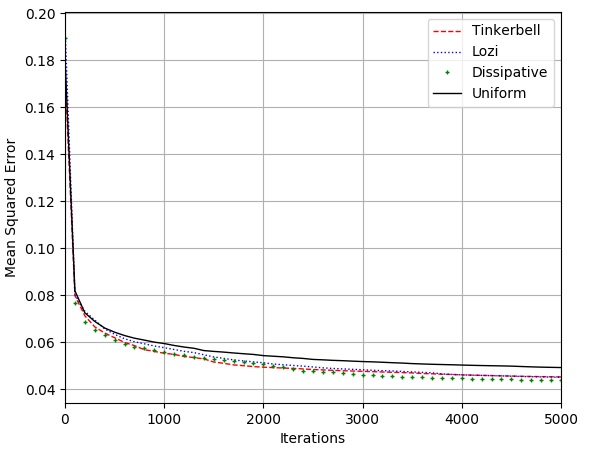
\includegraphics[width=90mm]{images/results/GbestGlassNone.png}}
\caption{$gBest$ topology- Glass Identification - $ E_T $ over 5000 iterations - No $ V_{max} $}
\label{fig:gbest:glass}
\end{figure}

\begin{figure}[htbp]
\centerline{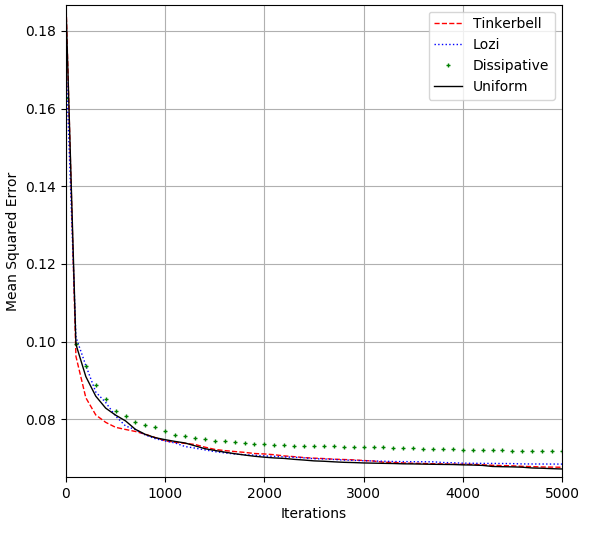
\includegraphics[width=90mm]{images/results/VNGlassNone.png}}
\caption{\ac{VN} topology- Glass Identification - $ E_T $ over 5000 iterations - No $ V_{max} $}
\label{fig:vn:glass}
\end{figure}

\begin{figure}[htbp]
\centerline{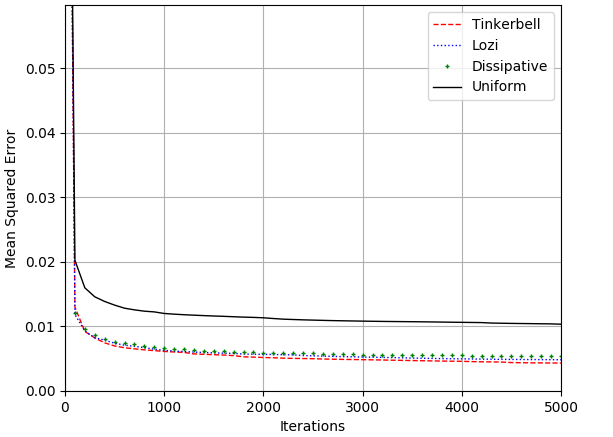
\includegraphics[width=90mm]{images/results/GbestIrisNone.png}}
\caption{$gBest$ topology- Iris - $ E_T $ over 5000 iterations - No $ V_{max} $}
\label{fig:gbest:iris}
\end{figure}

Fig. \ref{fig:gbest:iris} represents another more distinguishable result of this study where a \ac{CPSO}'s performance befit can be properly observed. The uniform \ac{PSO} is seen performing significantly worse than the \ac{CPSO} sampled from Tinkerbell, Lozi and Dissipative. While this result appears positive this is not an the general tendency over all experiments as can be observed in Fig. \ref{fig:vn:glass} and \ref{fig:vn:diabetes}.

\begin{figure}[htbp]
\centerline{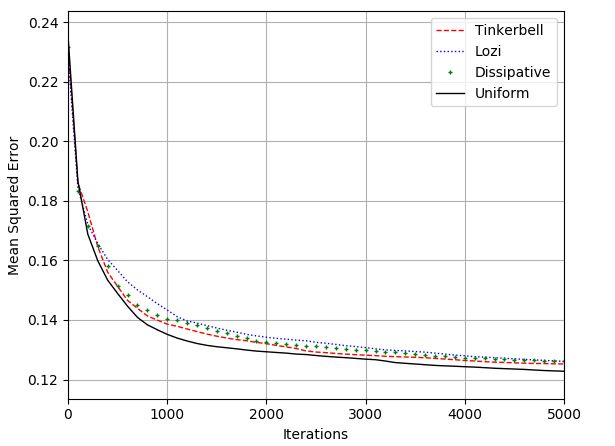
\includegraphics[width=90mm]{images/results/VNDiabetesNone.png}}
\caption{\ac{VN} topology- Diabetes - $ E_T $ over 5000 iterations - No $ V_{max} $}
\label{fig:vn:diabetes}
\end{figure}

The uniformly sampled \ac{PSO} in Fig. \ref{fig:gbest:heart} can be seen outperforming the other chaotic maps.

\begin{figure}[htbp]
\centerline{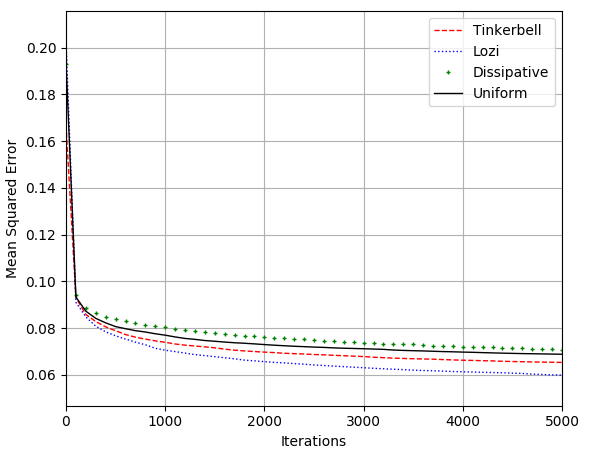
\includegraphics[width=90mm]{images/results/GbestHeartNone.png}}
\caption{$gBest$ topology- Heart - $ E_T $ over 5000 iterations - No $ V_{max} $}
\label{fig:gbest:heart}
\end{figure}

Lozi and Tinkerbell can be observed performing well in training in Fig. \ref{fig:gbest:heart}.

\newpage
\section{Conclusion}
In conclusion it is difficult to recommend a \ac{CPSO} as an improvement over a basic \ac{PSO} for \ac{NN} training. While a \ac{CPSO} does often allow for reduced \ac{NN} training and generalisation error in some cases this results in increased overfitting. Additionally \ac{CPSO}s may occasionally reduce training and generalisation error. A Basic \ac{PSO} sampled uniformly form $ (0, 1) $ resulted in performance difference that were statistically insignificant from a \ac{CPSO} in a significant amount of experiments.

Further research could involve applying \ac{CPSO}s to problems that require significantly higher number of weights.

\newpage

\nocite{*}
\noindent
\bibliographystyle{IEEEtran}
\indent
\bibliography{IEEEabrv,sbc-template}

\end{document}
